\subsection{複数の数を並べる}

制御対象には、一つの実数だけでは表せない量がある。平面上の位置は横方向と縦方向の二つの成分を持ち、モータの状態は電流、角速度、角度などの複数の成分で表される。複数の成分を順序付きに並べた量をベクトルとして扱う。

\begin{definition}[ベクトル]
複数の数を順序付きに並べたものをベクトルという。$n$ 個の実数成分を持つベクトルは $\R^n$ の元である。たとえば
\begin{equation}
  x=\begin{bmatrix}2\\3\end{bmatrix}
\end{equation}
は、1番目の成分が 2、2番目の成分が 3 のベクトルである。
\end{definition}

ベクトルは、複数の成分を一つの記号で表す記法である。平面上の位置は
\begin{equation}
  p=\begin{bmatrix}p_x\\p_y\end{bmatrix}
\end{equation}
と書ける。速度は
\begin{equation}
  v=\begin{bmatrix}v_x\\v_y\end{bmatrix}
\end{equation}
と書ける。位置と速度をまとめて状態として定義するなら
\begin{equation}
  x=\begin{bmatrix}p_x\\p_y\\v_x\\v_y\end{bmatrix}
\end{equation}
と並べればよい。

\subsubsection{ベクトル演算と座標}

ベクトルを物理量として使うときは、成分の順序だけでなく、各成分の単位も固定する。平面上の位置ベクトル
\begin{equation}
  p=\begin{bmatrix}p_x\\p_y\end{bmatrix}
\end{equation}
では、$p_x$ と $p_y$ は同じ座標系で測った長さであり、単位はいずれも m である。二つの位置ベクトル $p$ と $r$ が同じ座標系で表されているなら、和と差を成分ごとに定義できる。
\begin{align}
  p+r
  &=
  \begin{bmatrix}p_x+r_x\\p_y+r_y\end{bmatrix},\\
  p-r
  &=
  \begin{bmatrix}p_x-r_x\\p_y-r_y\end{bmatrix}.
\end{align}
和と差の各成分は m のままである。互いに異なる単位の量、たとえば位置 m と速度 $\mathrm{m/s}$ は、同じ物理ベクトルの成分として足すことはできない。

\begin{definition}[ベクトルの和とスカラー倍]
$a,b\in\R^n$ を
\begin{equation}
  a=\begin{bmatrix}a_1\\a_2\\\vdots\\a_n\end{bmatrix},
  \qquad
  b=\begin{bmatrix}b_1\\b_2\\\vdots\\b_n\end{bmatrix}
\end{equation}
とする。同じ番号の成分どうしを足したベクトル
\begin{equation}
  a+b=
  \begin{bmatrix}
    a_1+b_1\\
    a_2+b_2\\
    \vdots\\
    a_n+b_n
  \end{bmatrix}
\end{equation}
をベクトルの和という。実数または物理量の係数 $\alpha$ により各成分を掛けたベクトル
\begin{equation}
  \alpha a=
  \begin{bmatrix}
    \alpha a_1\\
    \alpha a_2\\
    \vdots\\
    \alpha a_n
  \end{bmatrix}
\end{equation}
をスカラー倍という。
\end{definition}

スカラー倍では、$\alpha$ が無次元なら単位は変わらない。$\alpha$ が単位を持つ物理量なら、成分の単位はその分だけ変わる。たとえば質量 $m$ と加速度ベクトル $a$ から
\begin{equation}
  F=ma
\end{equation}
と力ベクトルを作るとき、$m$ の単位は kg、$a$ の単位は $\mathrm{m/s^2}$ である。したがって $F$ の各成分の単位は
\begin{equation}
  \mathrm{kg}\cdot\frac{\mathrm{m}}{\mathrm{s^2}}
  =
  \mathrm{N}
\end{equation}
である。力のつり合い
\begin{equation}
  F_1+F_2+F_3=0
\end{equation}
では、三つの力ベクトルが同じ座標系で表され、すべて N の単位を持つことを仮定している。

座標系を固定すると、ベクトルは基底と座標の組で表される。平面の標準基底を
\begin{equation}
  e_x=\begin{bmatrix}1\\0\end{bmatrix},
  \qquad
  e_y=\begin{bmatrix}0\\1\end{bmatrix}
\end{equation}
とすると、位置ベクトルは
\begin{equation}
  p=p_x e_x+p_y e_y
\end{equation}
と書ける。ここで $e_x,e_y$ は方向を表す無次元のベクトルであり、係数 $p_x,p_y$ が m の単位を持つ。一般に、互いに平行でない二つの方向ベクトル $b_1,b_2$ を選ぶと、同じ位置を
\begin{equation}
  p=\xi_1 b_1+\xi_2 b_2
\end{equation}
の形で表せる場合がある。このとき $\xi_1,\xi_2$ が、その基底に関する座標である。物理的な位置 $p$ は同じでも、基底を変えれば座標の数値は変わる。状態空間でも同じで、状態ベクトルの成分は「対象そのもの」ではなく、選んだ座標で対象を表した数値である。

\begin{figure}[tb]
\centering
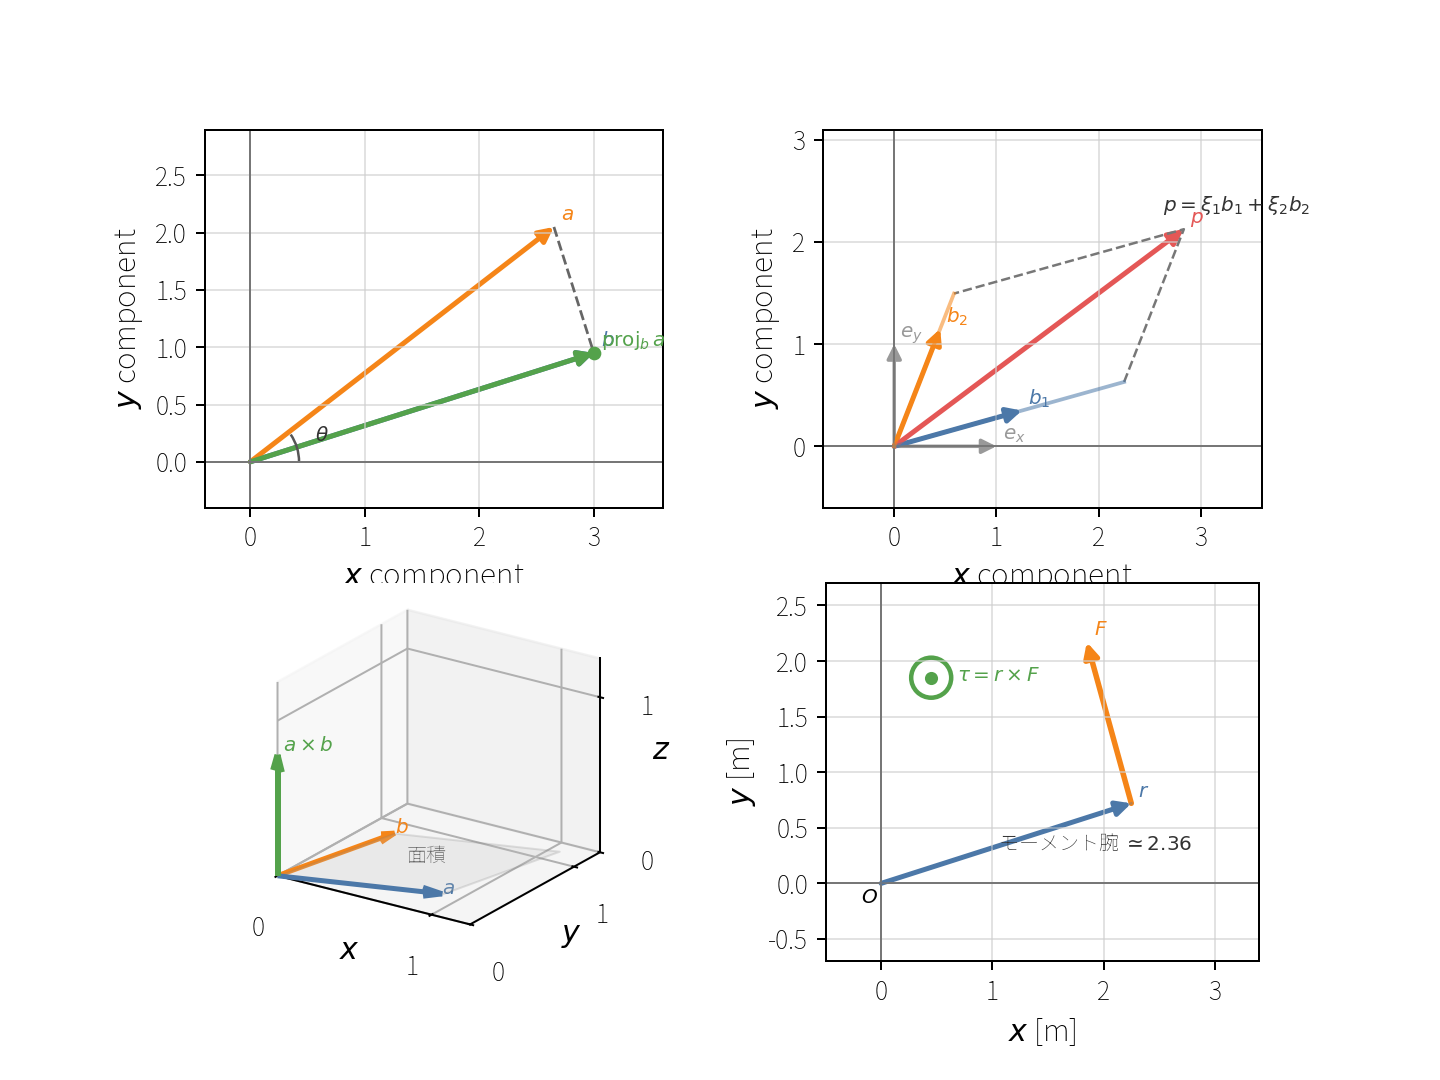
\includegraphics[width=0.94\linewidth,bb=0 0 1440 1080]{figures/vector_geometry_examples.png}
\caption{ベクトル、射影、基底、外積の幾何的関係。左上は内積が作る射影と直交成分を示す。右上は同じ点 $p$ が標準基底と斜めの基底で異なる座標成分を持つことを示す。左下は右手系で $a\times b$ が $a$ と $b$ の張る平面に垂直な向きを持つことを示す。右下は作用点ベクトル $r$ と力 $F$ から、回転軸まわりのモーメント $\tau=r\times F$ が決まることを示す。}
\label{fig:vector-projection-cross}
\end{figure}

図\ref{fig:vector-projection-cross} は、基底成分、射影、右手系、外積が作るモーメント方向を対応させている。以降の内積と外積は、この幾何的関係を成分計算へ移す演算として定義する。

\subsubsection{内積、ノルム、射影}

ベクトルの成分を足し合わせるだけでは、方向どうしの関係を数値にできない。力が変位と同じ向きを向いているか、速度が目標方向へ進んでいるか、状態偏差が評価関数のどの方向で大きいかを調べるには、二つのベクトルから一つの数を作る演算が必要になる。この役割を持つ基本演算が内積である。

\begin{definition}[内積]
$a,b\in\R^n$ に対して
\begin{equation}
  a^\T b
  =
  a_1b_1+a_2b_2+\cdots+a_nb_n
\end{equation}
を $a$ と $b$ の内積という。本文では列ベクトルを標準にするため、内積を $a^\T b$ と書く。
\end{definition}

内積の各項を足せるためには、各成分積 $a_i b_i$ が同じ単位を持つ必要がある。力 $F$ と変位 $d$ が同じ直交座標系で表されているなら、$F_i$ の単位は N、$d_i$ の単位は m であり、各項 $F_i d_i$ の単位は $\mathrm{N\,m}=\mathrm{J}$ でそろう。このとき
\begin{equation}
  W=F^\T d
\end{equation}
は、一定力 $F$ が変位 $d$ に対して行う仕事である。

二つのベクトルのなす角を $\theta$ とし、成分が同じ直交座標系で測られているとする。このとき内積は
\begin{equation}
  a^\T b=\norm{a}\norm{b}\cos\theta
\end{equation}
と書ける。したがって、内積が正なら $\theta<\pi/2$、負なら $\theta>\pi/2$、0 なら直交する。ここで使った $\norm{a}$ はベクトルの大きさである。

\begin{definition}[ユークリッドノルム]
$a\in\R^n$ に対して
\begin{equation}
  \norm{a}
  =
  \sqrt{a^\T a}
  =
  \sqrt{a_1^2+a_2^2+\cdots+a_n^2}
\end{equation}
を $a$ のユークリッドノルムという。
\end{definition}

位置ベクトルのノルムは原点からの距離であり、単位は m である。速度ベクトルのノルムは速さであり、単位は $\mathrm{m/s}$ である。一方、状態ベクトル
\begin{equation}
  x=\begin{bmatrix}q\\v\end{bmatrix}
\end{equation}
のように、成分が m と $\mathrm{m/s}$ で混在する場合、単純な $\sqrt{q^2+v^2}$ は物理量として意味を持たない。状態偏差の大きさを一つの数で測りたいときは、代表長さ $q_0$ と代表速度 $v_0$ を用いて
\begin{equation}
  \xi=
  \begin{bmatrix}
    q/q_0\\
    v/v_0
  \end{bmatrix}
\end{equation}
のように無次元化してから $\norm{\xi}$ を使う。LQR や Lyapunov 関数では、同じ目的のために重み行列を用いた二次形式 $x^\T Qx$ を使う。

\begin{definition}[射影]
$b\ne0$ とする。ベクトル $a$ の、$b$ が張る直線方向への射影を
\begin{equation}
  \operatorname{proj}_{b}a
  =
  \frac{a^\T b}{b^\T b}b
\end{equation}
で定義する。
\end{definition}

射影は、ある方向に沿った成分だけを取り出す操作である。力 $F$ のうち変位 $d$ の方向に効く成分は
\begin{equation}
  F_{\parallel}
  =
  \operatorname{proj}_{d}F
  =
  \frac{F^\T d}{d^\T d}d
\end{equation}
である。単位を確認すると、$F^\T d$ は J、$d^\T d$ は $\mathrm{m^2}$ なので、係数 $(F^\T d)/(d^\T d)$ の単位は $\mathrm{N/m}$ である。これに $d$ を掛けるため、$F_{\parallel}$ の単位は N になる。

\begin{example}[力、仕事、射影]
平面上で物体が
\begin{equation}
  d=\begin{bmatrix}3\\4\end{bmatrix}\,\mathrm{m}
\end{equation}
だけ移動し、一定力
\begin{equation}
  F=\begin{bmatrix}10\\0\end{bmatrix}\,\mathrm{N}
\end{equation}
を受けるとする。変位の大きさは
\begin{equation}
  \norm{d}=\sqrt{3^2+4^2}=5\,\mathrm{m}
\end{equation}
である。仕事は
\begin{align}
  W
  &=F^\T d\\
  &=10\cdot3+0\cdot4\\
  &=30\,\mathrm{J}.
\end{align}
変位方向の単位ベクトルを
\begin{equation}
  \hat{d}=\frac{d}{\norm{d}}
  =
  \begin{bmatrix}3/5\\4/5\end{bmatrix}
\end{equation}
とすると、力の変位方向成分の大きさは
\begin{equation}
  F^\T \hat{d}=10\cdot\frac{3}{5}=6\,\mathrm{N}
\end{equation}
である。したがって仕事は
\begin{equation}
  6\,\mathrm{N}\cdot5\,\mathrm{m}=30\,\mathrm{J}
\end{equation}
とも読める。力のうち移動方向と直交する成分は、この変位に対して仕事をしない。
\end{example}

状態空間でも、内積と射影は幾何的な意味を持つ。たとえば出力が
\begin{equation}
  y=c^\T x
\end{equation}
で表されるとき、$c$ は状態空間の中で測定が感度を持つ方向を指定している。状態の変化 $\Delta x$ が $c$ と直交すれば、一次近似では出力は変わらない。逆に $\Delta x$ が $c$ の方向成分を多く持てば、出力の変化は大きくなる。ただし、状態成分が異なる単位を持つときは、無次元化または適切な重みにより、内積の各項の単位をそろえてから解釈する。

\subsubsection{外積と力のモーメント}

三次元の力学では、回転を生む量を表すために外積を使う。内積が二つのベクトルの同じ向きの成分を数値化するのに対して、外積は二つのベクトルが張る平面に垂直な向きと、その面積に対応する大きさを持つベクトルを作る。

\begin{definition}[外積]
$a,b\in\R^3$ を
\begin{equation}
  a=\begin{bmatrix}a_1\\a_2\\a_3\end{bmatrix},
  \qquad
  b=\begin{bmatrix}b_1\\b_2\\b_3\end{bmatrix}
\end{equation}
とする。このとき
\begin{equation}
  a\times b
  =
  \begin{bmatrix}
    a_2b_3-a_3b_2\\
    a_3b_1-a_1b_3\\
    a_1b_2-a_2b_1
  \end{bmatrix}
\end{equation}
を $a$ と $b$ の外積という。
\end{definition}

外積 $a\times b$ は $a$ と $b$ の両方に直交する。二つのベクトルのなす角を $\theta$ とすると、大きさは
\begin{equation}
  \norm{a\times b}=\norm{a}\norm{b}\abs{\sin\theta}
\end{equation}
である。したがって、二つのベクトルが平行なら外積は 0 になり、直交すれば大きさが最大になる。向きは、選んだ座標系の右手系の規約に従う。

原点または回転軸から作用点までの位置ベクトルを $r$、作用する力を $F$ とする。力のモーメント、すなわちトルクは
\begin{equation}
  \tau=r\times F
\end{equation}
である。$r$ の単位が m、$F$ の単位が N なら、$\tau$ の単位は $\mathrm{N\,m}$ である。これは仕事の単位 J と同じ次元を持つが、トルクは回転軸まわりの向きを持つベクトル量として扱う。

\begin{example}[平面内の力が作るトルク]
回転軸を原点に置き、作用点が
\begin{equation}
  r=\begin{bmatrix}0.20\\0\\0\end{bmatrix}\,\mathrm{m}
\end{equation}
にあるとする。この点へ
\begin{equation}
  F=\begin{bmatrix}0\\15\\0\end{bmatrix}\,\mathrm{N}
\end{equation}
の力を加えると、
\begin{align}
  \tau
  &=r\times F\\
  &=
  \begin{bmatrix}
    0\cdot0-0\cdot15\\
    0\cdot0-0.20\cdot0\\
    0.20\cdot15-0\cdot0
  \end{bmatrix}\\
  &=
  \begin{bmatrix}0\\0\\3.0\end{bmatrix}\,\mathrm{N\,m}
\end{align}
である。平面内の力学では、この $z$ 成分
\begin{equation}
  \tau_z=r_xF_y-r_yF_x
\end{equation}
だけを扱うことが多い。振子、車輪、リンク機構のモデルでは、力そのものではなく、回転軸まわりのトルクが角加速度を決める。
\end{example}

図\ref{fig:vector-projection-cross} の四つの小図は、同じベクトル幾何を成分計算としても読めることを示している。左上の射影では、
\begin{align}
  b^\T\left(a-\operatorname{proj}_b a\right)
  &=
  b^\T a
  -
  b^\T\left(\frac{a^\T b}{b^\T b}b\right)\\
  &=
  b^\T a
  -
  \frac{a^\T b}{b^\T b}b^\T b\\
  &=0
\end{align}
となり、残差 $a-\operatorname{proj}_b a$ は $b$ と直交する。図の代表値として
$a=(2.65,2.05)^\T$、$b=(3.00,0.95)^\T$ を用いると、
\begin{equation}
  \operatorname{proj}_b a
  =
  \frac{9.8975}{9.9025}b
  \simeq
  \begin{bmatrix}2.998\\0.950\end{bmatrix}
\end{equation}
であり、点線で描かれた残差は射影先の緑の矢印と直角になる。右上では、同じ点が標準座標では
$p\simeq(2.84,2.13)^\T$ である一方、斜め基底では
\begin{equation}
  p=1.8b_1+1.3b_2
\end{equation}
と表されるため、座標成分は基底の選び方に依存する。左下では
$a\times b\simeq0.706e_z$ であり、順序を入れ替えると
$b\times a=-a\times b$ となって向きだけが反転する。右下のトルクも同じ外積で決まり、図の値では
\begin{equation}
  \tau_z=r_xF_y-r_yF_x
  =
  2.25\cdot1.45-0.72(-0.40)
  \simeq3.55\,\mathrm{N\,m}
\end{equation}
である。もし力の作用線が原点を通り $F=\lambda r$ と書けるなら、
$r_xF_y-r_yF_x=\lambda r_xr_y-\lambda r_yr_x=0$ となる。したがって図は、射影の残差が直交成分であること、座標値が基底に依存すること、外積の順序が向きを決めること、そして回転を生むのは力そのものではなく作用線から回転軸までの距離を含むモーメントであることを一続きに検算している。

\subsubsection{状態空間におけるベクトルの幾何}

状態空間では、状態を一つの点またはベクトルとして見る。直線上を動く質点の位置を $q$、速度を $v$ とし、状態を
\begin{equation}
  x=\begin{bmatrix}q\\v\end{bmatrix}
\end{equation}
と置く。このとき、状態空間の横軸を $q$、縦軸を $v$ とすれば、各時刻の状態は平面上の点である。質量 $m$ の質点に入力力 $u$ が加わり、摩擦を無視できると仮定すると、
\begin{equation}
  \dot{q}=v,
  \qquad
  \dot{v}=\frac{u}{m}
\end{equation}
である。したがって状態の時間変化は
\begin{equation}
  \dot{x}
  =
  \begin{bmatrix}
    v\\
    u/m
  \end{bmatrix}
\end{equation}
と書ける。$\dot{x}$ は状態空間上で、現在の点から次に進もうとする接線方向を表すベクトルである。

ただし、$q$ と $v$ は単位が異なるため、この平面の距離をそのままユークリッドノルムで測ることはできない。代表長さ $q_0>0$ と代表速度 $v_0>0$ を選び、
\begin{equation}
  \xi=
  \begin{bmatrix}
    q/q_0\\
    v/v_0
  \end{bmatrix}
\end{equation}
と無次元化すると、状態空間の幾何を数値的に比較しやすくなる。このとき
\begin{equation}
  \dot{\xi}
  =
  \begin{bmatrix}
    v/q_0\\
    u/(m v_0)
  \end{bmatrix}
\end{equation}
であり、各成分の単位は $1/\mathrm{s}$ でそろう。状態空間で距離、角度、射影を使うときは、どの座標で、どの単位または重みで測っているかを明示する必要がある。この注意が、後で状態フィードバック、可観測性、LQR の重み付けを読むときの基礎になる。

\subsubsection{行列と線形写像}

\begin{definition}[行列]
数を長方形に並べたものを行列という。たとえば
\begin{equation}
  A=\begin{bmatrix}1&2\\3&4\end{bmatrix}
\end{equation}
は 2 行 2 列の行列である。
\end{definition}

行列は、ベクトルからベクトルへの線形写像を表す。たとえば
\begin{equation}
  A=\begin{bmatrix}1&2\\3&4\end{bmatrix},
  \qquad
  x=\begin{bmatrix}5\\6\end{bmatrix}
\end{equation}
のとき、行列とベクトルの積は
\begin{align}
  Ax
  &=\begin{bmatrix}1&2\\3&4\end{bmatrix}
    \begin{bmatrix}5\\6\end{bmatrix}\\
  &=\begin{bmatrix}1\cdot5+2\cdot6\\3\cdot5+4\cdot6\end{bmatrix}\\
  &=\begin{bmatrix}17\\39\end{bmatrix}.
\end{align}
この積では、各行がベクトルの成分の重み付き和を定める。

一般に、$A\in\R^{m\times n}$ を
\begin{equation}
  A=
  \begin{bmatrix}
    a_{11}&a_{12}&\cdots&a_{1n}\\
    a_{21}&a_{22}&\cdots&a_{2n}\\
    \vdots&\vdots&\ddots&\vdots\\
    a_{m1}&a_{m2}&\cdots&a_{mn}
  \end{bmatrix}
\end{equation}
と書くと、$A$ は $n$ 個の成分を持つ入力ベクトル $x\in\R^n$ を、$m$ 個の成分を持つ出力ベクトル $y\in\R^m$ へ移す。
\begin{equation}
  y=Ax
\end{equation}
成分で書けば
\begin{equation}
  y_i=a_{i1}x_1+a_{i2}x_2+\cdots+a_{in}x_n
  =
  \sum_{j=1}^{n}a_{ij}x_j
\end{equation}
である。入力を二つ足してから写しても、それぞれを写してから足しても同じであり、係数を掛ける操作とも両立する。
\begin{align}
  A(x+r)&=Ax+Ar,\\
  A(\alpha x)&=\alpha Ax.
\end{align}
この性質を線形性という。行列は、有限個の成分で表された線形写像の表である。

物理量を行列で扱うときは、各成分の単位も同時に読む。状態
\begin{equation}
  x=\begin{bmatrix}q\\v\end{bmatrix}
\end{equation}
で、$q$ の単位が m、$v$ の単位が $\mathrm{m/s}$ であるとする。連続時間モデル
\begin{equation}
  \dot{x}=Ax
\end{equation}
の第 1 行が $\dot{q}$、第 2 行が $\dot{v}$ を与えるなら、$A$ の各成分は、掛ける状態成分の単位を対応する変化率の単位へ変換する単位を持つ。たとえば
\begin{equation}
  A=
  \begin{bmatrix}
    0&1\\
    -k/m&-c/m
  \end{bmatrix}
\end{equation}
では、$1$ は $v$ を $\dot{q}$ へ移す係数なので無次元ではなく、単位の換算を含めれば $\dot{q}$ と $v$ が同じ $\mathrm{m/s}$ を持つことを表している。$k/m$ の単位は $1/\mathrm{s^2}$、$c/m$ の単位は $1/\mathrm{s}$ であり、各項は $\dot{v}$ の単位 $\mathrm{m/s^2}$ にそろう。

\subsubsection{行列積と写像の合成}

行列を「ベクトルを別のベクトルへ移す規則」と読むと、行列積の意味が明確になる。$B\in\R^{n\times p}$ が $z\in\R^p$ を $x=Bz\in\R^n$ へ移し、$A\in\R^{m\times n}$ が $x$ を $y=Ax\in\R^m$ へ移すとする。この二つを続けて行うと
\begin{equation}
  y=A(Bz)
\end{equation}
である。この合成写像を一つの行列で表したものを $AB$ と書く。

\begin{definition}[行列積]
$A\in\R^{m\times n}$、$B\in\R^{n\times p}$ とする。$C=AB\in\R^{m\times p}$ の $(i,k)$ 成分を
\begin{equation}
  c_{ik}=
  \sum_{j=1}^{n}a_{ij}b_{jk}
\end{equation}
で定める。この $C$ を $A$ と $B$ の積という。
\end{definition}

積 $AB$ では、右側の $B$ が先に作用し、その後に左側の $A$ が作用する。したがって一般には
\begin{equation}
  AB\ne BA
\end{equation}
である。実際、そもそも $AB$ は定義できても $BA$ は寸法が合わず定義できないことがある。制御では、センサの座標変換、状態フィードバック、観測器、離散化、予測モデルの積を読むときに、この「右から順に作用する」という順序が重要になる。

\begin{example}[合成としての行列積]
まず平面ベクトルを
\begin{equation}
  B=
  \begin{bmatrix}
    2&0\\
    0&1
  \end{bmatrix}
\end{equation}
で横方向に 2 倍し、次に
\begin{equation}
  A=
  \begin{bmatrix}
    1&1\\
    0&1
  \end{bmatrix}
\end{equation}
で第 2 成分を第 1 成分へ加えるとする。合成は
\begin{align}
  AB
  &=
  \begin{bmatrix}
    1&1\\
    0&1
  \end{bmatrix}
  \begin{bmatrix}
    2&0\\
    0&1
  \end{bmatrix}\\
  &=
  \begin{bmatrix}
    2&1\\
    0&1
  \end{bmatrix}
\end{align}
である。たとえば $z=\begin{bmatrix}1\\3\end{bmatrix}$ なら
\begin{align}
  Bz&=\begin{bmatrix}2\\3\end{bmatrix},\\
  A(Bz)&=\begin{bmatrix}5\\3\end{bmatrix},\\
  (AB)z&=
  \begin{bmatrix}
    2&1\\
    0&1
  \end{bmatrix}
  \begin{bmatrix}1\\3\end{bmatrix}
  =
  \begin{bmatrix}5\\3\end{bmatrix}.
\end{align}
同じ結果が得られるので、$AB$ は「$B$ の後に $A$」を一つにまとめた行列である。
\end{example}

\subsubsection{逆行列と連立方程式}

正方行列 $A\in\R^{n\times n}$ が、ある行列 $A^{-1}$ により
\begin{equation}
  A^{-1}A=I,\qquad AA^{-1}=I
\end{equation}
を満たすとき、$A^{-1}$ を $A$ の逆行列という。ここで $I$ は単位行列であり、任意の $x$ に対して $Ix=x$ を満たす。

逆行列が存在するなら、連立一次方程式
\begin{equation}
  Ax=b
\end{equation}
は
\begin{align}
  A^{-1}Ax&=A^{-1}b,\\
  Ix&=A^{-1}b,\\
  x&=A^{-1}b
\end{align}
と解ける。したがって逆行列は、線形写像 $A$ によって変換された量から、もとの量を一意に戻す操作である。逆に、異なる二つのベクトル $x_1\ne x_2$ が同じ $Ax_1=Ax_2$ へ移るなら、出力から入力を一意に戻せないので逆行列は存在しない。

二次元では、行列
\begin{equation}
  A=
  \begin{bmatrix}
    a&b\\
    c&d
  \end{bmatrix}
\end{equation}
に対して
\begin{equation}
  \det A=ad-bc
\end{equation}
が 0 でないとき
\begin{equation}
  A^{-1}
  =
  \frac{1}{ad-bc}
  \begin{bmatrix}
    d&-b\\
    -c&a
  \end{bmatrix}
\end{equation}
である。分母 $ad-bc$ が 0 になる場合は、この式では逆行列を作れない。

連立方程式は、行列の式として読むだけでなく、行基本変形で読むこともできる。行基本変形とは、方程式の両辺に同じ操作を施して解集合を変えない変形であり、行の入れ替え、0 でない定数倍、別の行の定数倍を足す操作からなる。

\begin{example}[連立方程式を行基本変形で解く]
連立方程式
\begin{align}
  x_1+2x_2&=5,\\
  3x_1+4x_2&=11
\end{align}
を考える。拡大係数行列で書けば
\begin{equation}
  \left[
  \begin{array}{cc|c}
    1&2&5\\
    3&4&11
  \end{array}
  \right]
\end{equation}
である。第 2 行から第 1 行の 3 倍を引くと
\begin{equation}
  \left[
  \begin{array}{cc|c}
    1&2&5\\
    0&-2&-4
  \end{array}
  \right]
\end{equation}
となる。第 2 行を $-2$ で割ると
\begin{equation}
  \left[
  \begin{array}{cc|c}
    1&2&5\\
    0&1&2
  \end{array}
  \right]
\end{equation}
であり、第 1 行から第 2 行の 2 倍を引けば
\begin{equation}
  \left[
  \begin{array}{cc|c}
    1&0&1\\
    0&1&2
  \end{array}
  \right]
\end{equation}
を得る。したがって
\begin{equation}
  x=\begin{bmatrix}1\\2\end{bmatrix}
\end{equation}
である。係数行列
\begin{equation}
  A=
  \begin{bmatrix}
    1&2\\
    3&4
  \end{bmatrix}
\end{equation}
の行列式は $\det A=1\cdot4-2\cdot3=-2$ で 0 ではないので、二つの方程式は独立であり、解は一意に定まる。
\end{example}

\subsubsection{行列式、ランク、独立な方程式}

二次元の行列式は、面積の倍率として解釈できる。$A$ の第 1 列と第 2 列を
\begin{equation}
  a_1=\begin{bmatrix}a\\c\end{bmatrix},
  \qquad
  a_2=\begin{bmatrix}b\\d\end{bmatrix}
\end{equation}
とすると、$a_1$ と $a_2$ が張る平行四辺形の符号付き面積は
\begin{equation}
  \det A=ad-bc
\end{equation}
である。符号は向きの規約を表し、絶対値 $\abs{\det A}$ が面積倍率である。$\det A=0$ なら、単位正方形は面積 0 の線分または点へつぶれる。このとき、異なる入力が同じ出力へ重なり得るため、逆行列は存在しない。

三次元では行列式の絶対値が体積倍率を表す。一般の $n$ 次元でも、$\abs{\det A}$ は $n$ 次元体積の倍率であり、符号は向きの反転を表す。行列式は正方行列に対する量であり、長方形の行列では別の概念が必要になる。その役割を担うのがランクである。

\begin{definition}[ランク]
行列 $A$ の列ベクトルが張る空間の次元を $A$ のランクといい、$\operatorname{rank}A$ と書く。
\end{definition}

ランクは、行列が入力空間のうち何次元分の独立な方向を出力へ残しているかを表す。$A\in\R^{m\times n}$ に対して
\begin{equation}
  \operatorname{rank}A\le\min(m,n)
\end{equation}
である。正方行列 $A\in\R^{n\times n}$ では、$\operatorname{rank}A=n$ のとき、すべての方向がつぶれずに残り、逆行列が存在する。二次元ではこれは $\det A\ne0$ と同じ条件である。

連立方程式
\begin{equation}
  Ax=b
\end{equation}
では、$A$ の各行が一つの一次方程式を表す。行同士が独立であれば、各方程式は解を絞り込む新しい条件を与える。たとえば
\begin{equation}
  \begin{bmatrix}
    1&2\\
    2&4
  \end{bmatrix}
  x
  =
  \begin{bmatrix}
    5\\
    10
  \end{bmatrix}
\end{equation}
では、第 2 式は第 1 式の 2 倍であり、新しい条件を与えない。係数行列のランクは 1 で、未知数が 2 個あるため、解は一つに定まらず直線上に残る。一方、
\begin{equation}
  \begin{bmatrix}
    1&2\\
    2&4
  \end{bmatrix}
  x
  =
  \begin{bmatrix}
    5\\
    9
  \end{bmatrix}
\end{equation}
では、第 2 式の左辺は第 1 式の 2 倍なのに右辺は 2 倍ではないので、二つの条件は矛盾し、解は存在しない。ランクは、「独立な方程式がいくつあるか」と「写像の出力として到達できる方向が何次元あるか」を同時に表す。

\subsubsection{状態座標変換}

状態ベクトルの成分は、対象そのものではなく、選んだ座標で対象を表した数値である。したがって、同じ物理状態を別の座標で表すことがある。$T\in\R^{n\times n}$ が逆行列を持つとし、
\begin{equation}
  x=Tz
\end{equation}
で古い状態座標 $x$ と新しい状態座標 $z$ を結ぶ。このとき $T$ が逆行列を持つことは、$x$ と $z$ が一対一に対応し、状態の情報を失わないことを意味する。

状態方程式が
\begin{equation}
  \dot{x}=Ax+Bu
\end{equation}
で与えられているとする。$x=Tz$ と置き、$T$ が時間に依存しないと仮定すると
\begin{equation}
  \dot{x}=T\dot{z}
\end{equation}
である。これを状態方程式へ代入すると
\begin{align}
  T\dot{z}&=ATz+Bu,\\
  \dot{z}&=T^{-1}ATz+T^{-1}Bu.
\end{align}
したがって新しい座標での行列は
\begin{equation}
  A_z=T^{-1}AT,\qquad B_z=T^{-1}B
\end{equation}
である。出力方程式が
\begin{equation}
  y=Cx
\end{equation}
なら
\begin{equation}
  y=CTz
\end{equation}
なので、新しい出力行列は $C_z=CT$ である。

\begin{example}[状態の単位をそろえる座標変換]
状態
\begin{equation}
  x=\begin{bmatrix}q\\v\end{bmatrix}
\end{equation}
で、$q$ の単位が m、$v$ の単位が $\mathrm{m/s}$ であるとする。代表長さ $q_0>0$ と代表速度 $v_0>0$ を用いて
\begin{equation}
  z=
  \begin{bmatrix}
    q/q_0\\
    v/v_0
  \end{bmatrix}
\end{equation}
と無次元状態を作る。この関係は
\begin{equation}
  x=Tz,\qquad
  T=
  \begin{bmatrix}
    q_0&0\\
    0&v_0
  \end{bmatrix}
\end{equation}
と書ける。$q_0$ と $v_0$ が正なら
\begin{equation}
  T^{-1}=
  \begin{bmatrix}
    1/q_0&0\\
    0&1/v_0
  \end{bmatrix}
\end{equation}
が存在するので、無次元状態 $z$ から元の状態 $x$ へ、また $x$ から $z$ へ一意に戻れる。状態フィードバック、可観測性、LQR の重み付けでは、このような座標変換を行っても同じ物理状態を扱っていることを確認しながら、行列の形だけが変わる。
\end{example}

\subsubsection{固有値、固有ベクトル、モード座標}

行列は一般にはベクトルの向きも大きさも変える。しかし、特別な方向では、行列を掛けても向きが変わらず、大きさだけが変わることがある。このような方向は、状態空間の自然な動き、すなわちモードを読むための基準になる。

\begin{definition}[固有値と固有ベクトル]
正方行列 $A\in\R^{n\times n}$ に対して、$v\ne0$ と数 $\lambda$ が
\begin{equation}
  Av=\lambda v
\end{equation}
を満たすとき、$\lambda$ を $A$ の固有値、$v$ を $\lambda$ に対応する固有ベクトルという。
\end{definition}

固有ベクトルが表す直線上では、$A$ の作用は方向を変えず、伸縮だけになる。連続時間の自由応答
\begin{equation}
  \dot{x}=Ax
\end{equation}
を考え、初期値が固有ベクトル方向
\begin{equation}
  x(0)=\alpha v
\end{equation}
にあるとする。$x(t)=\beta(t)v$ と置くと
\begin{align}
  \dot{x}(t)&=\dot{\beta}(t)v,\\
  Ax(t)&=\beta(t)Av
    =\beta(t)\lambda v
\end{align}
である。したがって
\begin{equation}
  \dot{\beta}(t)=\lambda\beta(t)
\end{equation}
となり、
\begin{equation}
  x(t)=\alpha e^{\lambda t}v
\end{equation}
を得る。この意味で、固有ベクトルは不変な方向、固有値はその方向の増減率である。$\lambda<0$ ならそのモードは指数的に減衰し、$\lambda>0$ なら指数的に増大する。複素固有値の場合は、実部が包絡の増減率、虚部が振動角周波数に対応する。この対応は、後で極、二次遅れ、状態空間の安定性を読むときに同じ形で現れる。

固有ベクトルを十分な本数だけ選べる場合、行列の作用はモードごとに分解できる。互いに独立な固有ベクトル $v_1,\ldots,v_n$ があり、それぞれの固有値を $\lambda_1,\ldots,\lambda_n$ とする。行列
\begin{equation}
  T=\begin{bmatrix}v_1&v_2&\cdots&v_n\end{bmatrix},
  \qquad
  D=\diag(\lambda_1,\lambda_2,\ldots,\lambda_n)
\end{equation}
を作ると、
\begin{equation}
  AT=TD
\end{equation}
である。$T$ が逆行列を持つなら
\begin{equation}
  T^{-1}AT=D
\end{equation}
となる。この形に変形できることを対角化という。状態方程式 $\dot{x}=Ax$ に対して
\begin{equation}
  x=Tz
\end{equation}
と置くと、
\begin{align}
  T\dot{z}&=ATz,\\
  \dot{z}&=T^{-1}ATz,\\
  \dot{z}&=Dz
\end{align}
である。成分ごとに書けば
\begin{equation}
  \dot{z}_i=\lambda_i z_i
\end{equation}
となり、各モードは互いに独立な一次方程式として読める。対角化できない行列では、このような完全な分離はできず、後でジョルダン標準形や数値的な固有値計算の注意が必要になる。

\subsubsection{二次形式と正定値行列}

状態の大きさ、偏差の重み、機械エネルギー、リアプノフ関数、LQR の評価関数はいずれも、二次式として表されることが多い。ベクトル $x\in\R^n$ と正方行列 $P\in\R^{n\times n}$ に対して
\begin{equation}
  x^\T P x
\end{equation}
を $P$ が定める二次形式という。

二次形式をエネルギーや大きさとして使うときは、通常 $P$ が対称であることを仮定する。実際、任意の $P$ に対して
\begin{equation}
  P_s=\frac{1}{2}(P+P^\T)
\end{equation}
と置くと、
\begin{equation}
  x^\T P x=x^\T P_s x
\end{equation}
である。これは、反対称な部分 $P-P^\T$ が二次形式には寄与しないためである。したがって、正定値性を議論するときは対称行列を基準にする。

\begin{definition}[正定値行列と半正定値行列]
対称行列 $P=P^\T$ に対して、すべての $x\ne0$ で
\begin{equation}
  x^\T P x>0
\end{equation}
が成り立つとき、$P$ を正定値行列といい、$P\succ0$ と書く。すべての $x$ で
\begin{equation}
  x^\T P x\ge0
\end{equation}
が成り立つとき、$P$ を半正定値行列といい、$P\succeq0$ と書く。
\end{definition}

対角行列
\begin{equation}
  P=\diag(p_1,p_2,\ldots,p_n)
\end{equation}
では、
\begin{equation}
  x^\T P x=p_1x_1^2+p_2x_2^2+\cdots+p_nx_n^2
\end{equation}
である。したがって、すべての $p_i$ が正なら $P\succ0$、すべての $p_i$ が 0 以上なら $P\succeq0$ である。対称行列については、スペクトル定理により、長さ 1 で互いに直交する固有ベクトルを並べた行列 $U$ と実固有値を並べた対角行列 $\Lambda$ によって
\begin{equation}
  P=U\Lambda U^\T
\end{equation}
と書ける。$z=U^\T x$ と置けば
\begin{equation}
  x^\T P x
  =
  z^\T \Lambda z
  =
  \lambda_1z_1^2+\lambda_2z_2^2+\cdots+\lambda_nz_n^2
\end{equation}
である。したがって、対称行列の正定値性は、すべての固有値が正であることと同値である。半正定値性は、すべての固有値が 0 以上であることに対応する。

\begin{figure}[tb]
\centering
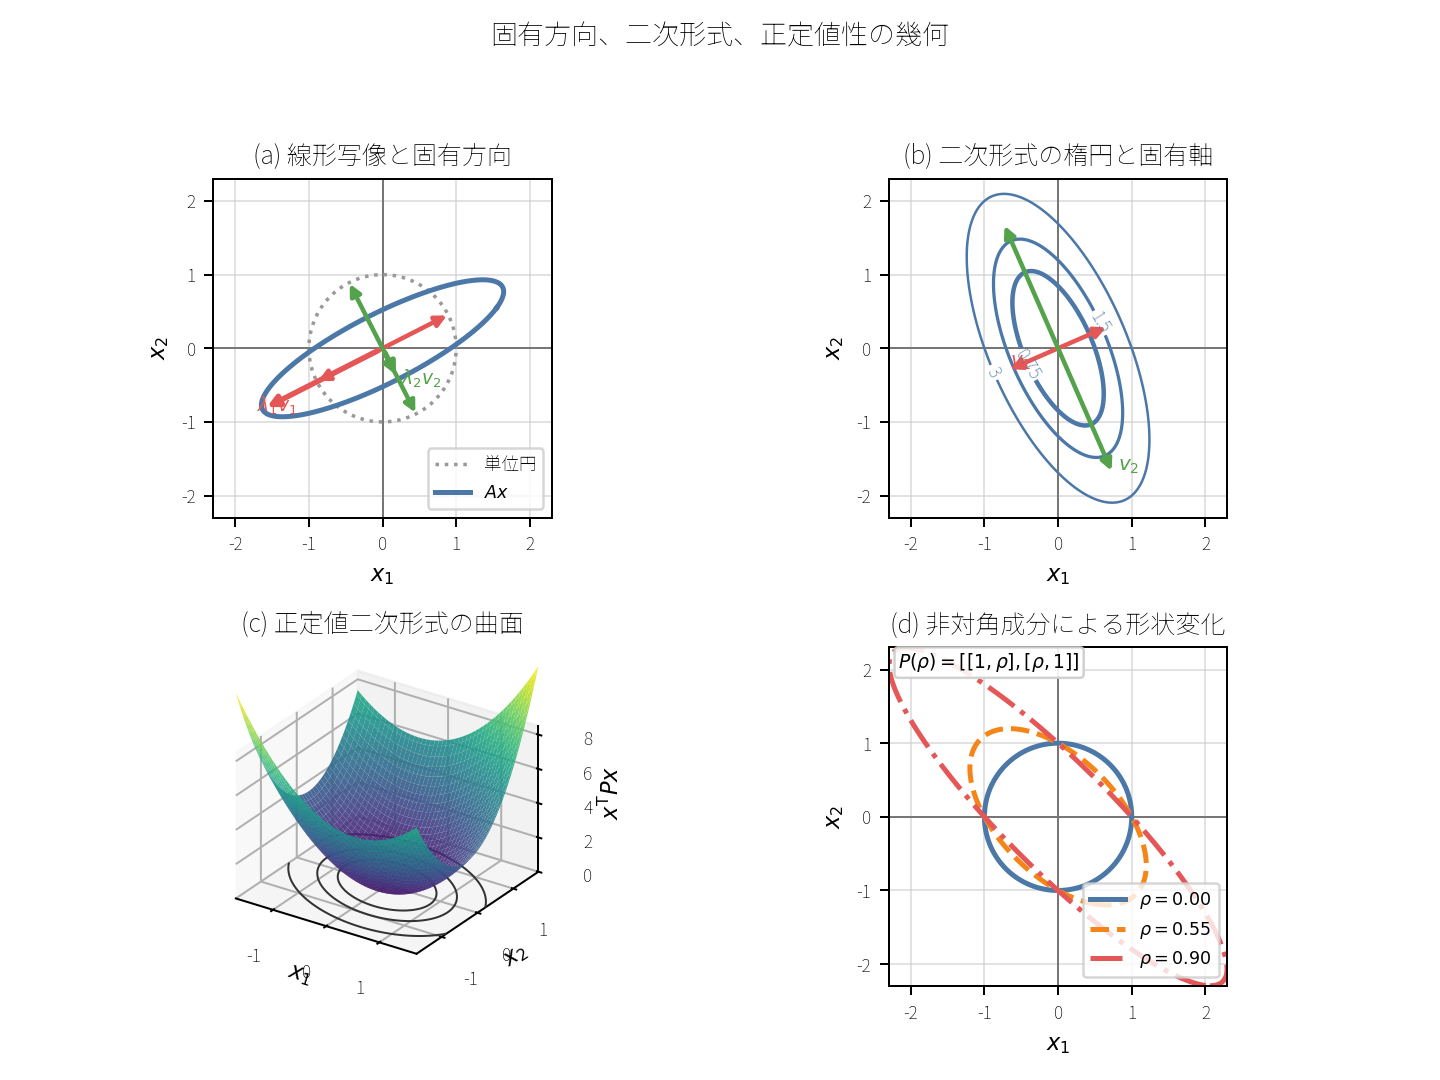
\includegraphics[width=0.94\linewidth,bb=0 0 1440 1080]{figures/linear_algebra_geometry_examples.png}
\caption{固有方向、二次形式、正定値性の幾何的関係。左上は線形写像 $A$ が一般の方向を曲げる一方、固有ベクトル方向では伸縮だけを与えることを示す。右上は $x^\T Px=\mathrm{const.}$ の楕円と固有軸を対応させている。左下は正定値二次形式が原点を底とする曲面を作ることを示す。右下は非対角成分 $\rho$ を大きくすると楕円が傾き、ある方向が強く罰せられることを示す。}
\label{fig:linear-algebra-geometry-examples}
\end{figure}

図\ref{fig:math-entrance-examples} 右下は、二つの正定値行列が作る等高線 $x^\T Px=\mathrm{const.}$ を比較している。$P=I$ ではどの方向も同じ重みなので等高線は円になる。非対角成分を持つ重み行列では、楕円の軸が座標軸から回転し、細い方向の状態偏差が強く罰せられる。この幾何は、後で LQR の重み、Lyapunov 関数、正規分布の共分散楕円を解釈する際の基準になる。
図\ref{fig:linear-algebra-geometry-examples} は、この見方を固有方向と曲面まで広げている。対称行列では固有ベクトルが二次形式の主軸になり、固有値が大きい方向ほど同じ値に達するまでの距離が短くなる。したがって、正定値性を確認することは、すべての方向で評価またはエネルギーが負にならず、原点から離れると正の値を持つことを確認する操作である。

機械系のエネルギーは、正定値行列の最も標準的な例である。ばね定数 $k>0$、質量 $m>0$ の一次元質量ばね系で、平衡位置からの変位を $q$、速度を $v$ とすると、位置エネルギーと運動エネルギーの和は
\begin{equation}
  E(q,v)=\frac{1}{2}kq^2+\frac{1}{2}mv^2
\end{equation}
である。状態を
\begin{equation}
  x=\begin{bmatrix}q\\v\end{bmatrix}
\end{equation}
と置けば、
\begin{equation}
  E(x)=\frac{1}{2}x^\T
  \begin{bmatrix}
    k&0\\
    0&m
  \end{bmatrix}
  x
\end{equation}
である。$k$ と $m$ が正なので、この行列は正定値であり、原点以外の状態ではエネルギーが正になる。

リアプノフ関数も同じ構造を使う。原点を平衡点とする線形系
\begin{equation}
  \dot{x}=Ax
\end{equation}
に対して、
\begin{equation}
  V(x)=x^\T P x,\qquad P\succ0
\end{equation}
を候補に選ぶと、$V(x)$ は原点で 0、原点以外で正になる。時間微分は
\begin{align}
  \dot{V}
  &=\dot{x}^\T P x+x^\T P\dot{x}\\
  &=(Ax)^\T P x+x^\T P(Ax)\\
  &=x^\T A^\T P x+x^\T P A x\\
  &=x^\T(A^\T P+PA)x
\end{align}
である。ここで $M\preceq0$ は $-M\succeq0$ を意味し、すべての $x$ で $x^\T Mx\le0$ となることを表す。もし $A^\T P+PA\preceq0$ なら、$V$ は時間とともに増えない。さらにすべての $x\ne0$ で $x^\T(A^\T P+PA)x<0$ になる場合は、原点から離れた状態で $V$ が厳密に減少する。この考えが、後で扱うリアプノフ安定性、リアプノフ方程式、LQR の重み行列へつながる。LQR の評価
\begin{equation}
  J=\int_0^\infty \left(x^\T Qx+u^\T Ru\right)\,\dd t
\end{equation}
では、通常 $Q\succeq0$、$R\succ0$ を仮定し、状態偏差と入力の二乗評価が負の報酬にならないようにする。

\begin{example}[二次系のモードとエネルギー]
無次元化済みの二次系
\begin{equation}
  \dot{x}=Ax,\qquad
  A=
  \begin{bmatrix}
    0&1\\
    -2&-3
  \end{bmatrix},
  \qquad
  x=\begin{bmatrix}q\\v\end{bmatrix}
\end{equation}
を考える。固有値は
\begin{align}
  \det(\lambda I-A)
  &=
  \det
  \begin{bmatrix}
    \lambda&-1\\
    2&\lambda+3
  \end{bmatrix}\\
  &=\lambda(\lambda+3)+2\\
  &=(\lambda+1)(\lambda+2)
\end{align}
より、$\lambda_1=-1$、$\lambda_2=-2$ である。対応する固有ベクトルとして
\begin{equation}
  \phi_1=
  \begin{bmatrix}1\\-1\end{bmatrix},
  \qquad
  \phi_2=
  \begin{bmatrix}1\\-2\end{bmatrix}
\end{equation}
を選べる。したがって
\begin{equation}
  T=\begin{bmatrix}1&1\\-1&-2\end{bmatrix},
  \qquad
  T^{-1}AT=
  \begin{bmatrix}
    -1&0\\
    0&-2
  \end{bmatrix}
\end{equation}
であり、$x=Tz$ と置けば
\begin{equation}
  \dot{z}_1=-z_1,\qquad
  \dot{z}_2=-2z_2
\end{equation}
となる。第 2 モードは第 1 モードより速く減衰する。

同じ系に対して
\begin{equation}
  E(q,v)=q^2+\frac{1}{2}v^2
  =
  \frac{1}{2}x^\T
  \begin{bmatrix}
    2&0\\
    0&1
  \end{bmatrix}
  x
\end{equation}
を考える。この重み行列は正定値である。軌道に沿って微分すると
\begin{align}
  \dot{E}
  &=2q\dot{q}+v\dot{v}\\
  &=2qv+v(-2q-3v)\\
  &=-3v^2\\
  &\le0
\end{align}
となる。エネルギー型の二次形式は増えず、固有値は二つのモードがいずれも減衰することを示している。このように、モードによる時間率の読み取りと、正定値二次形式によるエネルギー評価は、安定性を別々の角度から確認する道具である。
\end{example}

図\ref{fig:math-entrance-examples} と図\ref{fig:linear-algebra-geometry-examples} は、微積分の局所量と二次形式の幾何を同じ「近傍での変化の読み取り」としてつないでいる。図\ref{fig:math-entrance-examples} 左上では、$h$ を小さくすると二点を結ぶ割線の傾きが操作点の接線の傾き、すなわち微分係数に近づく。左下では $r(t)<0$ の区間の符号付き面積が負であるため、累積量はその区間で減少する。右上では一次 Taylor 近似の誤差は操作点の近くで小さく、離れるほど曲率の影響で大きくなるので、線形化を使うときは操作点と有効範囲を本文中で固定しておく必要がある。右下では赤い破線の楕円が青い円より細い方向ほど、同じ二次形式値を保つために許される状態偏差が小さい。したがって、その方向は重み行列によって強く罰せられる方向である。

図\ref{fig:linear-algebra-geometry-examples} 右上の楕円も同じ事実を固有値で表している。対称正定値行列を $P=V\Lambda V^\T$、$V^\T x=y$ と対角化すると、
\begin{equation}
  x^\T Px
  =
  \lambda_1y_1^2+\lambda_2y_2^2
\end{equation}
である。等高線 $x^\T Px=c$ の半径は固有方向 $v_i$ に沿って $\sqrt{c/\lambda_i}$ になるため、大きい固有値に対応する方向が短軸になる。右下の $\rho$ を含む二次形式では、交差項が固有方向を標準座標軸から斜め方向へ回し、$|\rho|$ が大きいほど等高線は細くなる。$\rho$ の符号を変えると、細く伸びる向きも反対側の対角方向へ入れ替わる。
